\begin{figure}[htbp]
\centering 
  \subfloat[Box plot \acs{SCT}.]{
	  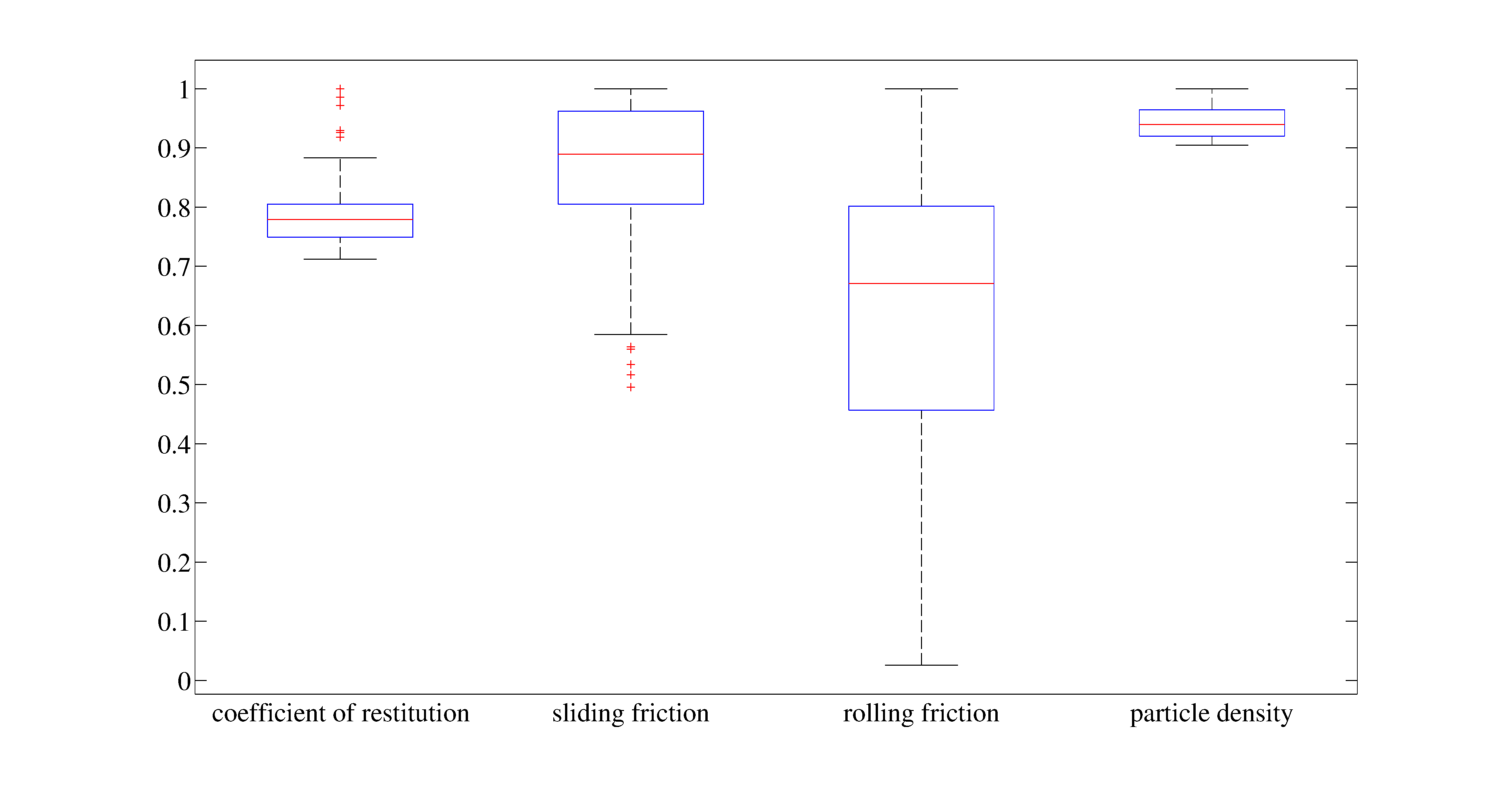
\includegraphics[width=.47\columnwidth]{images/168BoxSCTironorecoarsetest01coeffP1}
	  \label{fig:168BoxSCTironorecoarsetest01coeffP1}
  }
  \quad
  \subfloat[Density plot \acs{SCT}.]{
	  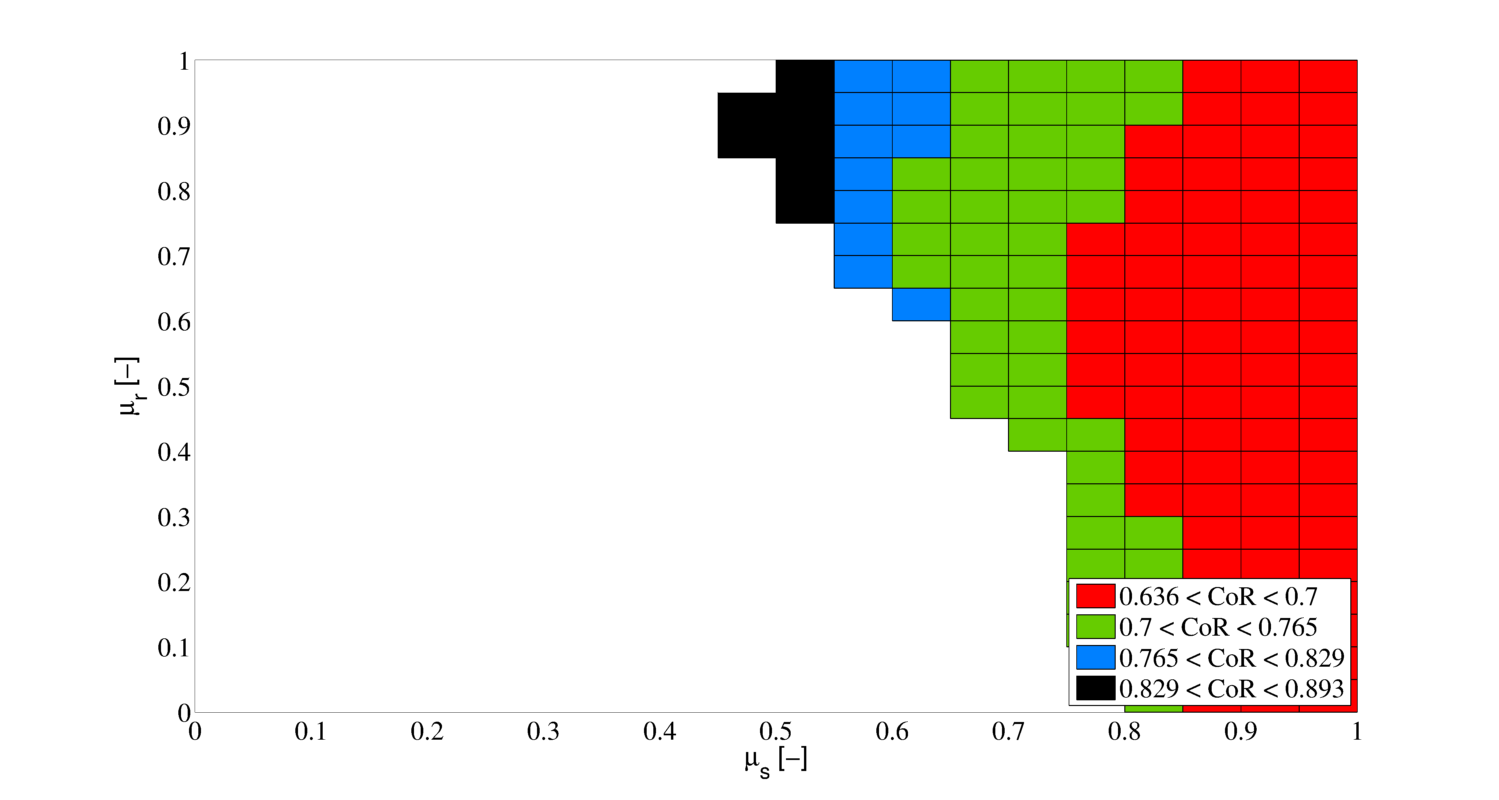
\includegraphics[width=.47\columnwidth]{images/174TileSCironorecoarsetest01coeffP1}
	  \label{fig:174TileSCironorecoarsetest01coeffP1}
  }
  \\
    \subfloat[Box plot \acs{AoR}.]{
	  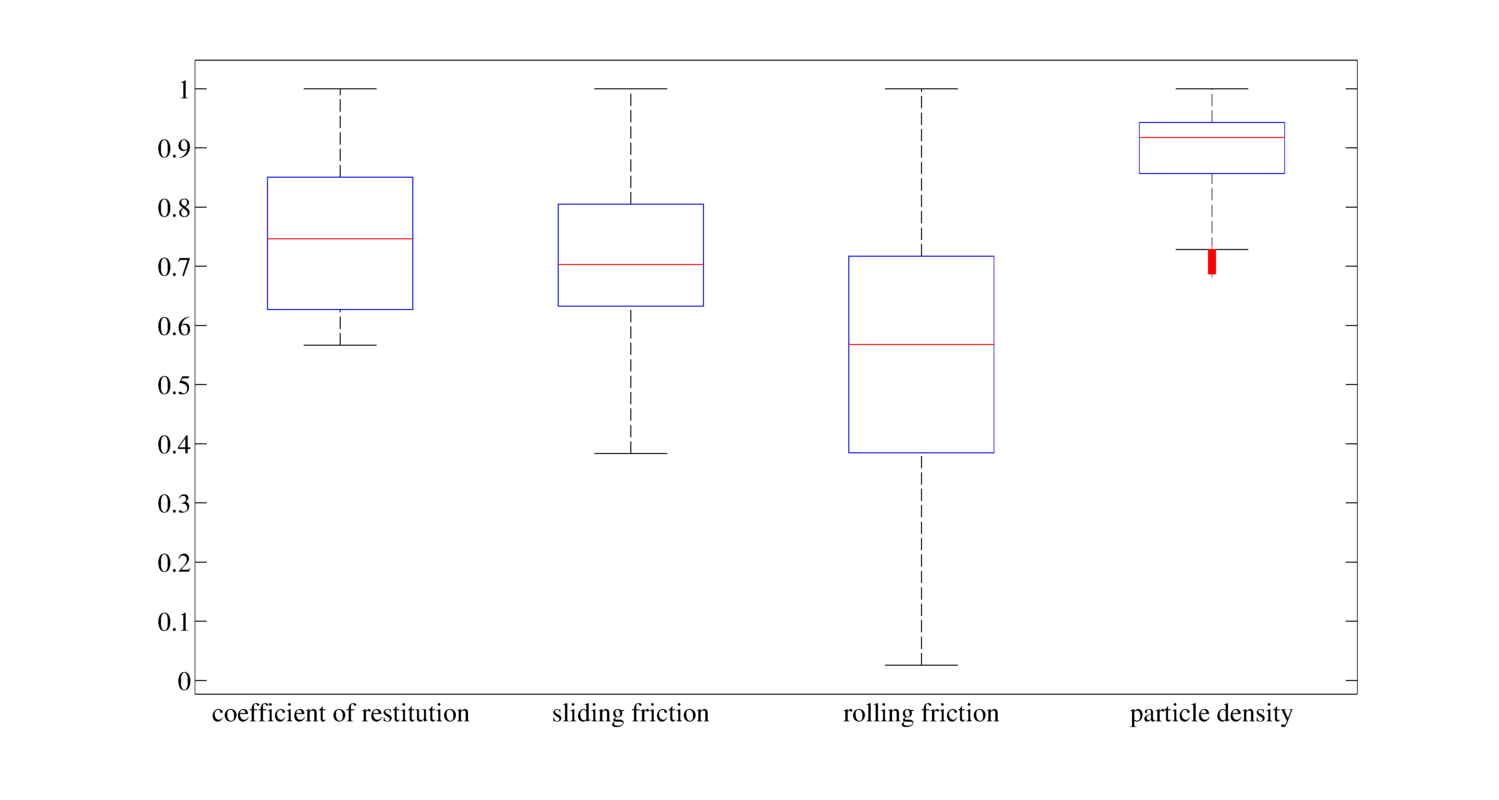
\includegraphics[width=.47\columnwidth]{images/181BoxAORironorecoarse}
	  \label{fig:181BoxAORironorecoarse}  }
  \quad
  \subfloat[Density plot \acs{AoR}.]{
	  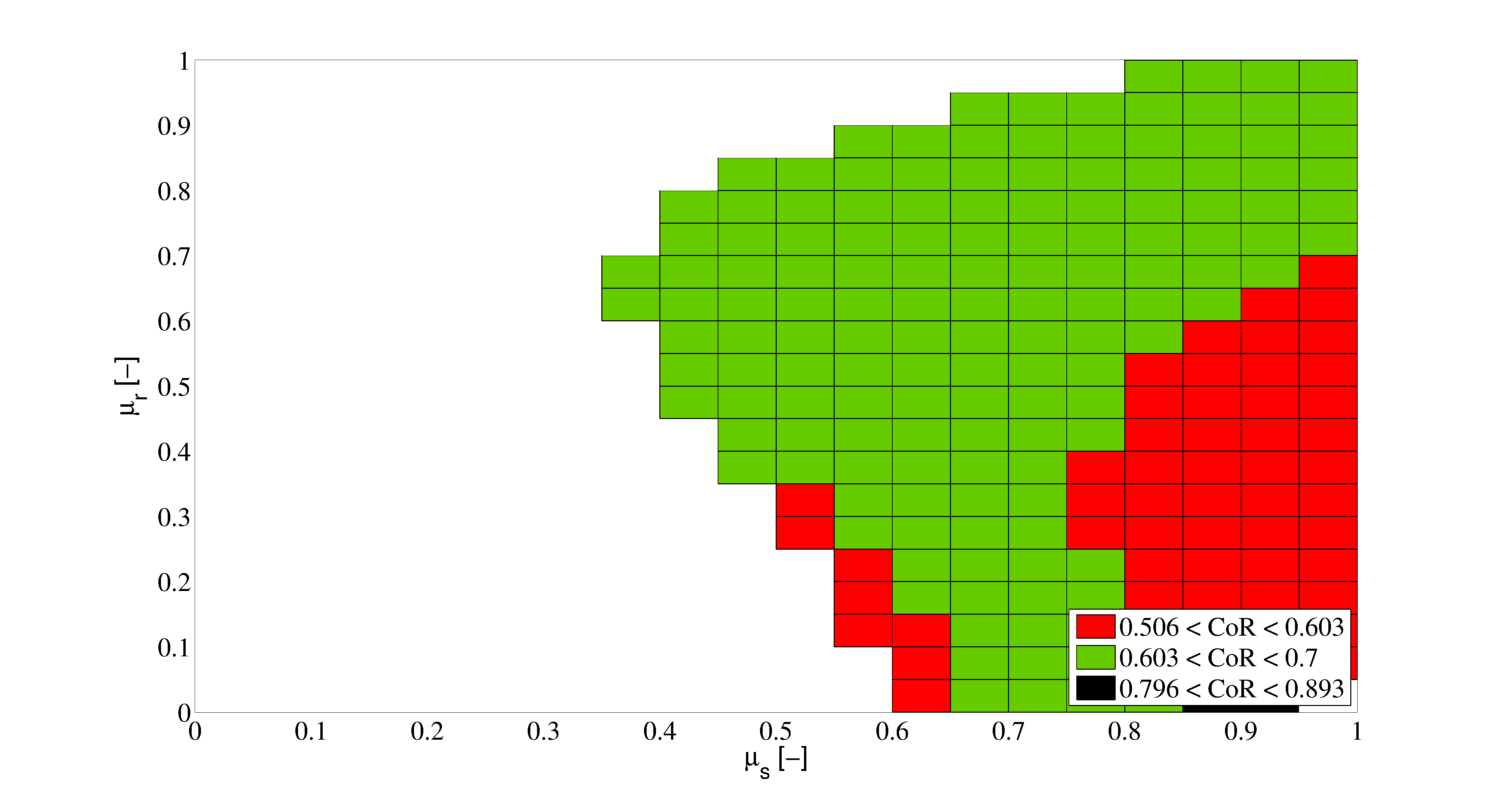
\includegraphics[width=.47\columnwidth]{images/182TileAORironorecoarse}
	  \label{fig:182TileAORironorecoarse}  }
  \\
  \subfloat[Box plot intersection: \acs{AoR} \& \acs{SCT}.]{
	  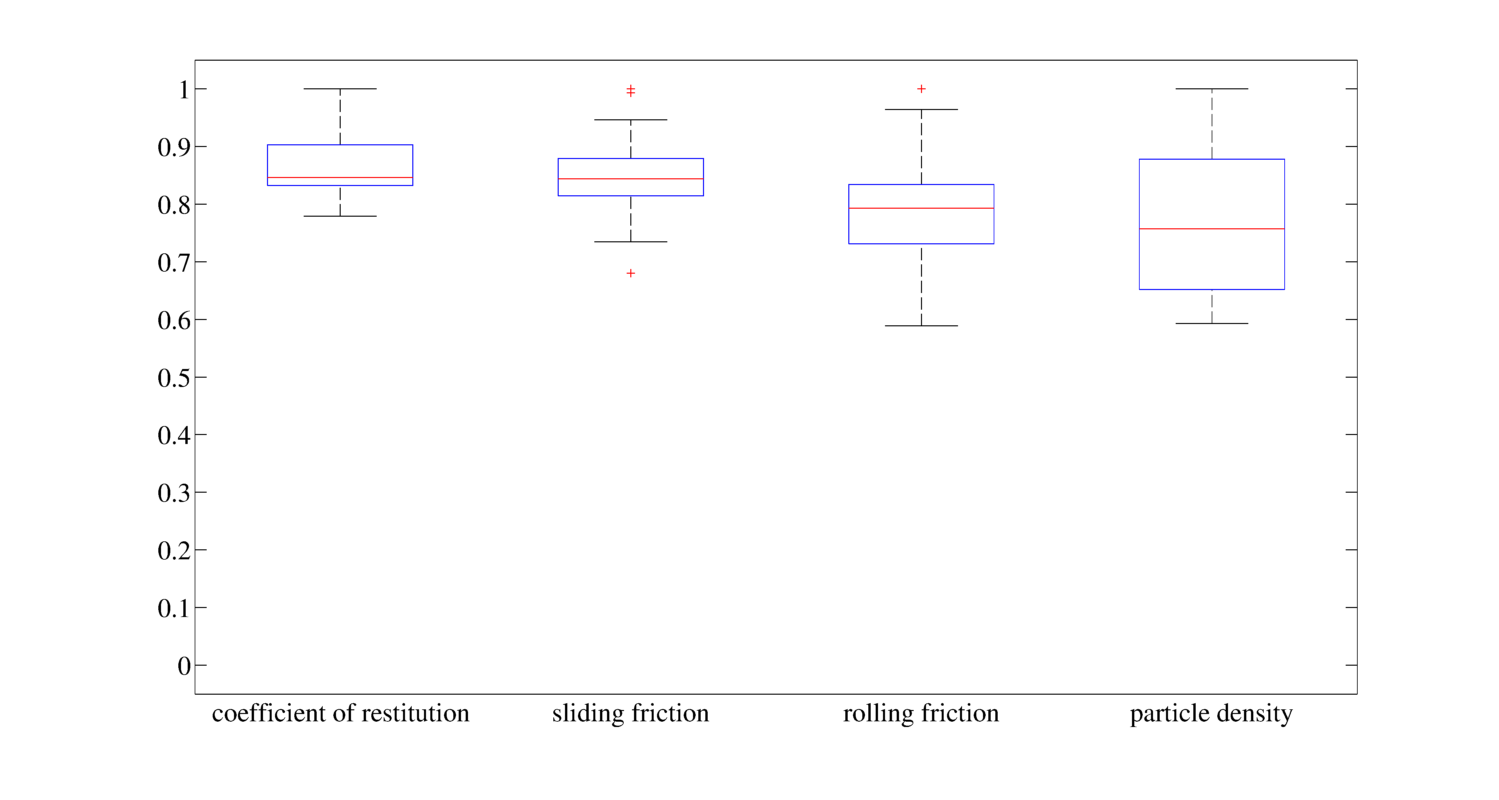
\includegraphics[width=.47\columnwidth]{images/199BoxMixironorecoarse_28}
	  \label{fig:199BoxMixironorecoarse_28}
  }
  \quad
  \subfloat[Density plot intersection: \acs{AoR} \& \acs{SCT}.]{
	  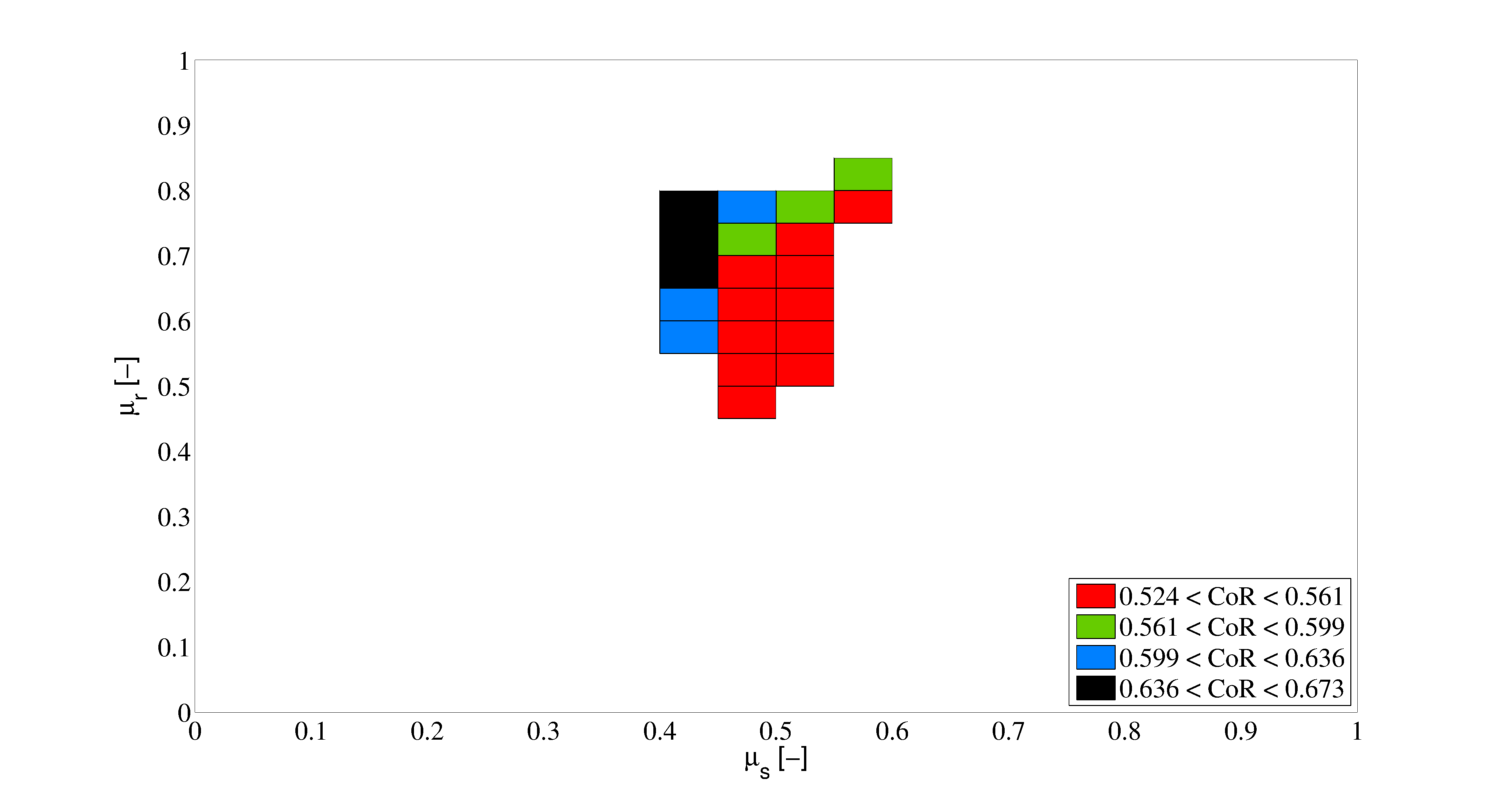
\includegraphics[width=.47\columnwidth]{images/200TileMixironorecoarse_28}
	  \label{fig:200TileMixironorecoarse_28}
  }
  \\    
  \caption{Iron ore coarse.}
  \label{fig:213boxplotsironorecoarse}
\end{figure}